\documentclass[border=4pt]{standalone}
\usepackage{amsmath,amssymb,tikz}
\usetikzlibrary{arrows.meta}
\begin{document}
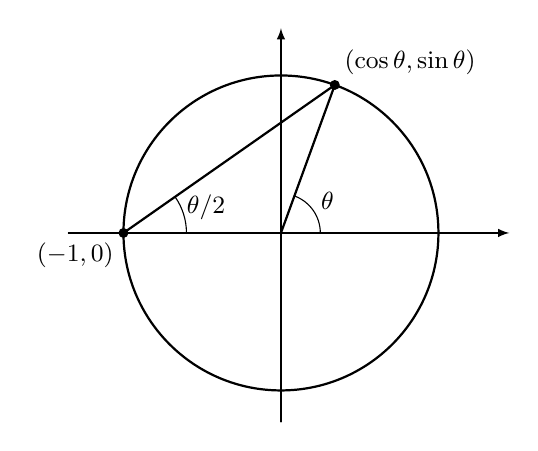
\begin{tikzpicture}[scale=2.0,>=latex,line cap=round]
  \def\th{70}
  \draw[->] (-1.35,0) -- (1.45,0);
  \draw[->] (0,-1.2) -- (0,1.3);
  \draw[thick] (0,0) circle (1);
  \draw[thick] (-1,0) -- ({cos(\th)},{sin(\th)});
  \draw[thick] (0,0) -- ({cos(\th)},{sin(\th)});
  \draw (0.25,0) arc (0:\th:0.25); \node[font=\small] at ({0.36*cos(\th/2)},{0.36*sin(\th/2)}) {$\theta$};
  \draw (-0.6,0) arc (0:\th/2:0.4); \node[font=\small] at ({-1+0.55*cos(\th/4)},{0.55*sin(\th/4)}) {$\theta/2$};
  \fill (-1,0) circle (0.9pt) node[below left,font=\small]{$(-1,0)$};
  \fill ({cos(\th)},{sin(\th)}) circle (0.9pt) node[above right,font=\small]{$(\cos\theta,\sin\theta)$};
\end{tikzpicture}
\end{document}
